\documentclass[11pt]{article}

\usepackage[T1]{fontenc}
\usepackage[margin=1.15in]{geometry}
\usepackage{amsmath,amssymb,amsthm}
\usepackage{setspace}
\usepackage{booktabs}
\usepackage{longtable}
\usepackage{tikz}
\usetikzlibrary{positioning}
\usepackage[colorlinks=true,linkcolor=black,citecolor=black,urlcolor=black]{hyperref}

\setstretch{1.12}
\setlength{\parskip}{0.55em}
\setlength{\parindent}{0pt}

\newtheorem{hypothesis}{Hypothesis}
\renewcommand{\thehypothesis}{H\arabic{hypothesis}}
\newtheorem{proposition}{Proposition}
\theoremstyle{definition}
\newtheorem{definition}{Definition}

\newcommand{\R}{\mathbb{R}}
\newcommand{\E}{\mathbb{E}}
\newcommand{\F}{\mathcal{F}}
\newcommand{\Hmap}{\mathcal{H}}
\newcommand{\Pmap}{\mathcal{P}}

\title{Programmable Material Organization:\\
Process History, Structural Constraint, and Functional Manufacturing\\[0.4em]
\large A Research Program in the Control of Internal State During Fabrication}
\author{Flyxion\\Independent Researcher}
\date{October 2026}

\begin{document}
\maketitle

\begin{abstract}
\noindent Additive and solution-based manufacturing are usually described in terms of the geometries they can produce. A growing body of experimental work indicates that this description omits the variables that most often determine what a manufactured object does. Crystallographic continuity, molecular orientation, dislocation and precipitate gradients, pore connectivity across length scales, and the chemical environment established by an apparatus are all properties of a fabricated state that is set by a process history and is largely invisible in the external shape. This essay develops a research program around that observation.

\noindent A common state-space vocabulary is introduced for the description of fabricated material, a process operator is defined that maps manufacturing inputs and environmental histories to final internal states, and a functional operator maps those states to measurable performance under stated operating conditions. Within this vocabulary a set of structural propositions is stated, including the non-identifiability of function from geometry, the distinction between order and uniformity, the conditions under which local corrective operations improve a growing structure, and the diminishing returns of serial transport optimization. A statistical notion of task-relative sufficiency is then defined for manufacturing records, which converts the question of how much process history must be retained into one that experiments can answer. Seven complementary research strands, linked by a shared vocabulary and two designated transfer tests, are then specified, each with hypotheses, experimental designs, performance measures, and explicit conditions under which the hypothesis would be abandoned. The program is organized around liquid-crystalline elastomers, hierarchically porous sorbents, metallic single crystals with engineered gradients, organic semiconductor films and crystals, and printed chemical apparatus, but is formulated so that the methodology, and not the particular material systems, carries the generality. Throughout, the aim is to preserve the physical differences among material classes while building a shared discipline of modeling, measurement, record keeping, and validation.
\end{abstract}

\tableofcontents
\newpage

%--------------------------------------------------------------------
\section{Introduction}

The conventional account of digital fabrication treats the object as a geometric specification realized in a material. A computer model describes surfaces and volumes, a slicing procedure converts the model into a sequence of toolpaths, and a machine deposits or consolidates matter along those paths. Quality is then assessed by dimensional accuracy, surface finish, and the absence of gross defects such as voids or delamination. Under this account the material is a relatively passive carrier of the geometry, and the principal engineering question is how faithfully the machine can reproduce the intended shape.

This account has always been incomplete, because the properties that make engineered materials useful are rarely properties of shape. The strength and creep resistance of a metallic component depend on grain structure, dislocation density, precipitate distribution, and residual stress. The charge mobility of an organic semiconducting film depends on molecular packing and the connectivity of ordered domains. The actuation of a liquid-crystalline polymer depends on the director field that was frozen into it during processing. The uptake kinetics of a porous sorbent depend on the coordination of transport pathways spanning several orders of magnitude in length. In each case the property of interest belongs to an internal organization that is established during fabrication, and two objects that are indistinguishable by external measurement may differ in that organization sufficiently to behave in opposite ways.

Recent experimental work has made it difficult to regard this fact as a secondary complication. Wire-arc deposition with pulsed remelting has been used to grow metallic single crystals up to a meter in length and in complex architected geometries, which implies that crystallographic continuity can be maintained through a process that is, by its nature, a repeated nucleation hazard \cite{liu2026,rohrer2026}. Printed smectic liquid-crystalline elastomers have been shown to switch the sign of their actuation strain according to the temperature and shear conditions under which they were extruded, so that identical toolpaths yield contraction or elongation \cite{lee2026}. Hierarchically porous sorbent monoliths have been printed with coordinated channel architectures that improve sorption and desorption kinetics by more than an order of magnitude over randomly packed material, and the same work found that the kinetic gain from a fourth hierarchical order was smaller than that from a third, which, together with the difficulty of printing the finer structure, led to a third-order design \cite{bai2026}. Spatial gradients of dislocation density, precipitates, and composition in additively manufactured single crystals have been quantified and associated with simultaneous gains in strength and ductility \cite{guo2025}. Earlier studies had already shown that printed polymer structures can embed light-driven molecular reorientation \cite{vanoosten2009}, that printed vessels can alter the distribution of chemical products through their geometry \cite{symes2012}, and that solution deposition can organize organic semiconductors into films or crystals with transport properties approaching those of ideal single crystals \cite{niazi2015,rigas2016}. These results span materials, scales, and mechanisms, and they are cited here as instances of a common pattern rather than as a closed corpus. The pattern is that the control variable of interest has moved from the boundary of the object to the interior of the material.

The purpose of this essay is to formulate a research program that takes that movement seriously. The program has three components. The first is a conceptual one: a vocabulary and a small set of formal statements that make precise what it means to manufacture an internal state, what is lost when only geometry is recorded, and which assumptions are needed before a process can be optimized against a functional target. The second is an experimental one: a set of strands of investigation, each tied to a measurable material system, that test the formal statements and that generate the data required to build predictive process models. The third is methodological: a proposal for how heterogeneous experimental efforts can share a record format, a validation discipline, and a vocabulary for reporting negative and null results, so that cumulative knowledge about process-dependent function becomes possible across laboratories and material classes.

That manufacturing conditions influence material function is long established and is not the claim advanced here. The more specific question is whether compact, transferable representations of manufacturing history can be identified and validated across apparatuses and material systems. The formal development proceeds from the observation that geometry is an insufficient record of a process, through a statement of what a sufficient record would be, to experiments that estimate how much of a process history must be retained for a given function to be predicted.

The scope is deliberately wide but the claims are deliberately restricted. The material systems involved are governed by different constitutive laws and are studied by different communities with different instruments. Crystallographic growth, mesogen alignment under shear, vapor diffusion in porous media, and reaction selectivity in a mixed flow are not special cases of a single physical theory, and the shared formalism offered here is not intended to suggest otherwise. It is a bookkeeping language that makes explicit what must be specified, measured, and tested, and the substantive physics is supplied by system-specific models. A program that treated mathematical resemblance as evidence of mechanistic unity would produce attractive analogies and little knowledge, and the temptation to do so is greatest precisely where the formalisms coincide most closely. The discipline proposed here is the opposite: to use a shared language in order to locate precisely where the systems differ. The principal risk of the program is accordingly that its unification proves rhetorical, and the criteria of Section~\ref{sec:limits} state in advance the evidence that would show this and the point at which the program should be reduced to separate studies.

%--------------------------------------------------------------------
\section{The Experimental Landscape as a Set of Worked Examples}

Before the formalism is introduced, it is useful to describe the experimental territory that motivates it. The following subsections are not a systematic review. Each presents one class of result in enough detail to show which variables of internal state were manipulated, what was measured, and what the result does and does not establish.

\subsection{Crystallographic continuity under repeated heating}

Conventional single-crystal growth relies on a stable directional thermal gradient maintained over long times, so that a single seed propagates through a melt or vapor while competing nuclei are suppressed. Wire-arc additive manufacturing operates in an almost opposite regime, in which small volumes are repeatedly heated and cooled, solidification fronts change direction continually, and the opportunity for stray nucleation is large. The authors identify three obstacles specific to additive manufacturing: the loss of the quasi-steady thermal field that directional solidification requires, the loss of the convex liquid-solid interface that favours single-crystal growth, and the incompatibility between microscopic growth conditions and the fabrication of large overhanging structures. The demonstration that meter-tall titanium alloy rods, lattices with zigzag ligaments, and several refractory metals and alloys (tungsten, molybdenum, niobium, and molybdenum-niobium) can be grown as single crystals under such conditions rests on alternating and pulsed heat inputs \cite{liu2026}. In the account given in the accompanying commentary, a wire is melted onto the previous layer at low current, after which a short high-current burst of about half a second spreads the deposit over the whole surface and remelts a thin volume of the layer beneath it, and the current is then lowered for a resolidification interval of about nine and a half seconds \cite{rohrer2026}. During resolidification the existing lattice templates the new material while misoriented grains formed on the surface are eliminated, a mechanism the commentary describes as self-correction. The notable feature is that the process does not prevent every deviation but corrects deviations repeatedly after they arise. The reported creep resistance of the titanium alloy exceeds by an order of magnitude the prediction obtained from the grain-size dependence of the steady-state creep rate in polycrystals, and the authors attribute this to two contributions acting together: the elimination of grain boundaries and an additive-manufacturing-induced hierarchical alpha and beta architecture that regulates dislocation density, mobility, and void evolution \cite{liu2026}. The resulting state therefore differs from a polycrystal in kind and not only in degree, and it is a state that is ordered in orientation while remaining internally structured.

An independent commentary adds a necessary qualification \cite{rohrer2026}. The commentary notes that the titanium alloy solidifies in a cubic lattice but transforms to a hexagonal structure on cooling, that the interfaces between the resulting phase variants can have properties similar to grain boundaries, and that this may be problematic for some applications. The same commentary reports that the crystal diameter is currently limited to between 6 and 20 millimeters. A solid-state transformation on cooling can therefore generate crystallographic variants and interfaces between them even when the high-temperature growth has been single-crystalline. A claim of single-crystal continuity at growth temperature therefore does not entail the absence of mechanically significant internal boundaries at service temperature. This distinction between the state established during growth and the state that persists to operation is a recurring theme in what follows, and it motivates the explicit separation of process states from functional states in the formalism.

\subsection{Organization of transport pathways in organic semiconductors}

Two lines of work on solution-processed organic semiconductors illustrate that a functional target can be reached by different structural routes. Blade coating of blends of a small-molecule semiconductor (diF-TES-ADT) with amorphous insulating polymers produces thin-film transistors with carrier mobility as high as $6.7\,\mathrm{cm^{2}\,V^{-1}\,s^{-1}}$, threshold voltages below $1\,\mathrm{V}$, and subthreshold swings below $0.5\,\mathrm{V\,dec^{-1}}$, while the films remain polycrystalline \cite{niazi2015}. The authors attribute the result to careful control over phase separation and crystallization, and they report that blends with different insulating polymers performed differently even though the thermodynamic driving forces for phase separation were expected to be nearly identical, which indicates that the morphology realized during coating, and not the nominal composition, carries the functional information. Spray deposition combined with antisolvent crystallization and solution shearing produces isolated organic single crystals at room temperature in air, on a wide range of substrates, with size, shape, and orientation controlled by the shear generated when spray droplets strike the antisolvent surface \cite{rigas2016}. In the first case the structure is an organized polycrystal whose boundaries do not obstruct transport appreciably. In the second case the structure is a set of isolated single crystals. The same engineering objective of high mobility is achieved in both, which establishes that the mapping from function back to structure is not one to one.

\subsection{Frozen molecular order and programmable actuation}

Liquid-crystalline polymer networks convert molecular order into mechanical response. When the order is changed by light or heat, the network deforms. Inkjet printing of self-organizing liquid-crystal inks containing photo-isomerizing azo compounds demonstrated that the order and the responsive chemistry can be placed spatially so as to produce artificial cilia whose subunits, printed from different inks, are addressed selectively by different wavelengths of light \cite{vanoosten2009}. More recent work with a smectic direct-ink-writing ink shows that shear and temperature can determine whether molecular alignment falls parallel or perpendicular to the print direction. Rheological, X-ray, and molecular dynamics analyses indicate that the inversion arises from the preservation or collapse of smectic layers under flow, with the collapse occurring above a critical shear rate and being most readily triggered near the transition temperature. As a consequence the thermal actuation strain of printed filaments ranges from elongation to substantial contraction, from about $+8.4\%$ to $-25.7\%$ as print speed is increased at $40\,^{\circ}$C, and a representative specimen retained its behavior over 100 heating and cooling cycles \cite{lee2026}. The significance of this result for the present argument is that toolpath geometry, which a conventional description would regard as sufficient to specify the object, does not determine the response. The response is determined jointly by the path and by the rheological and thermal conditions under which the path was traversed.

\subsection{Heterogeneity as a design variable}

A natural reading of the metallic single-crystal results would be that the ideal manufactured metal is one from which all internal variation has been removed. The analysis of internal gradients in additively manufactured single crystals shows that this reading is too simple \cite{guo2025}. Spatial variations in dislocation density, precipitate size and distribution, and composition around dendritic structures can be described by parametrized profiles and incorporated into mechanical simulations, and suitable combinations of such variations, described by a unified trigonometric function, appear to improve strength and ductility together, particularly at elevated temperature. The authors report that, in high-throughput simulations, mechanical properties correlate linearly with the intensity of the gradient, so that strength and elongation can be tuned by tuning it, whereas conventional gradient microstructures that require post-treatment raise strength at the expense of ductility. This weakens the habitual assumption of a strength-ductility trade-off as an inevitability and makes the more precise claim that the trade-off depends on how internal heterogeneity is organized. The relevant property of the material is therefore not its uniformity but the compatibility of its distributed internal structure with the intended loading.

\subsection{Coordination of transport across scales}

Printed hierarchical sorbents for atmospheric water harvesting combine macroscopic channels that carry bulk vapor flow with finer porosity in which diffusion and sorption occur \cite{bai2026}. The reported improvement in sorption and desorption kinetics over randomly packed material is large, twelvefold and fourteenfold respectively, but the more instructive findings concern the limits of architecture. The authors find that porosity and volumetric kinetics trade off against each other, so that medium porosity with low tortuosity is preferred, and that a four-order channel hierarchy raised the effective diffusion coefficient to 28.4 times that of a zero-order structure (a computed effective-diffusion measure, distinct from the twelvefold and fourteenfold kinetic improvements measured against randomly packed material) while its kinetic gain over the three-order structure was smaller than the three-order gain over the two-order one, which they ascribe to limited space and diffusion depth in high-order channels. Considering also the difficulty of printing four-order structures, they select the three-order design. The heat post-processing step additionally activates nanoscale and microscale porosity, so that the macroscale channels and the finer pore networks are produced by different stages of one process. This is a concrete instance of a general constraint on multiscale design, namely that the benefit of improving transport at one scale is bounded by the resistance remaining at the others. The same work is candid about unresolved issues of throughput, cost, energy demand, and feedstock sustainability, and those caveats are essential to any interpretation of reported productivity.

\subsection{Fabrication as part of the experiment}

Printed reaction vessels with integrated catalytic and analytical features show that the geometry of an apparatus can alter the distribution of products from nominally identical reagents \cite{symes2012}. The reported shift in dominant product between two apparatus designs does not mean that geometry overrides chemical kinetics. It means that mixing, residence time, surface contact, and local concentration are controlled partly by the apparatus, and that these variables enter the effective rate expressions. The example is conceptually important because it dissolves the boundary between making and measuring. The apparatus is both an object that has been fabricated and an instrument whose configuration is an experimental variable.

%--------------------------------------------------------------------
\section{A Formal Vocabulary for Manufactured State}

\subsection{State, process, and response}

Let $\Omega\subset\R^3$ denote the region occupied by a fabricated object and let $\mathbf{x}\in\Omega$ be a material point. The condition of the object is described by two kinds of variable that behave differently and are therefore kept apart. The slow structural state is
\begin{equation}
z(\mathbf{x},t)=\bigl(\phi,\ \mathbf{n},\ \rho_d,\ c,\ \psi,\ \sigma_r,\ \mathcal{G}\bigr)(\mathbf{x},t),
\end{equation}
whose components denote, respectively, local phase fractions, molecular or crystallographic orientation, dislocation density, chemical composition, porosity, residual stress, and a description of local connectivity. The fast field variables are $w(\mathbf{x},t)=(T,\sigma_a)$, the instantaneous temperature and the applied or transient stress, which are driven largely by boundary conditions and relax on time scales short compared with structural change. Residual stress is assigned to the structural state because it persists once the driving conditions are removed, whereas the instantaneous temperature and stress fields do not. The components are placeholders. A particular system uses the subset that is physically meaningful for it and may add others, such as defect type, interface character, or degree of cure. The only structural requirement is that $z$, together with the field variables fixed by the environment, be rich enough that the functional response of the object is determined.

The evolution of the structural state during fabrication is described schematically by
\begin{equation}
\frac{\partial z}{\partial t}=\F\bigl(z,\nabla z,\nabla^{2} z,w;\,u,\theta\bigr)+\eta,
\label{eq:evolution}
\end{equation}
where $\nabla^{2}$ acts componentwise on the vector-valued field, $u(t)$ collects controllable manufacturing inputs such as deposition rate, thermal schedule, electrical current, illumination, solvent composition, nozzle geometry, and deposition order, $\theta$ collects material parameters, and $\eta$ represents disturbances and unresolved dynamics. The field variables obey their own balance laws, such as heat conduction and momentum balance, driven by $u$, the boundary conditions, and the current structural state. Equation~\eqref{eq:evolution} is not a model of any particular process. It is a placeholder that states the minimal assumption: that the structural state evolves under the influence of controllable inputs, local interactions, the field variables, and noise. Different material systems substitute different operators for $\F$, including phase-field dynamics, rheological models of ordered fluids, reaction-diffusion systems, and heat conduction with moving boundaries.

The final structural state is the result of integrating this evolution along a process trajectory. Writing $e(t)$ for the environmental history to which the object is exposed during fabrication and $p=(z_0,u(\cdot),e(\cdot))$ for the process, one has
\begin{equation}
z_f=\Pmap[p]=\Pmap\bigl[z_0,\,u(\cdot),\,e(\cdot)\bigr],
\end{equation}
where $\Pmap$ is the process evolution operator and $z_0$ is the initial state, which includes the substrate or feedstock. The functional response under operating environment $e_{\mathrm{op}}$, which supplies the field variables during service, is
\begin{equation}
y=\Hmap\bigl(z_f,\,e_{\mathrm{op}}\bigr).
\end{equation}
Three questions are thereby separated that a geometry-centered description tends to merge: what external shape has been produced, what internal state has been established, and what that state does under actual operating conditions.

\subsection{Geometry as a projection}

Let $\pi$ denote the projection from the full state to the external geometry, so that the geometric description of the object is $g=\pi(z_f)$. A conventional digital model records $g$ and, at most, a nominal composition. The relation between geometry and function is then the composition $\Hmap\circ\Pmap$ restricted to those trajectories that yield the geometry $g$.

\begin{definition}[Geometric and functional equivalence]
Two processes $p_1$ and $p_2$ are geometrically equivalent, written $p_1\sim_g p_2$, if $\pi(\Pmap[p_1])=\pi(\Pmap[p_2])$, and functionally equivalent under the operating environment $e_{\mathrm{op}}$, written $p_1\sim_y p_2$, if $\Hmap(\Pmap[p_1],e_{\mathrm{op}})=\Hmap(\Pmap[p_2],e_{\mathrm{op}})$.
\end{definition}

Both are equivalence relations on the set of processes, and each geometric class is partitioned by the functional relation into classes that may be numerous.

\begin{proposition}[Geometric equivalence does not imply functional equivalence]
\label{prop:nonid}
If there exist processes $p_1\sim_g p_2$ with $p_1\not\sim_y p_2$, then no function of the geometry $g$ alone can predict the response $y$ for this system.
\end{proposition}

\begin{proof}
A function $f$ of $g$ must assign a single value to $g$. The two processes give the same $g$ and different $y$, so $f(g)$ cannot equal both. \qedhere
\end{proof}

The proposition is trivial as mathematics and consequential as engineering, because the existence of such pairs is demonstrated experimentally. Two filaments deposited along the same path but under different thermal and shear conditions have been shown to display opposite signs of actuation strain \cite{lee2026}, and metallic parts of the same shape with different thermal histories will differ in grain structure and residual stress. The proposition identifies the requirement that follows. Wherever the history is consequential, the digital description of an object has to carry information beyond geometry, and the necessary information is determined by the dimension of the state that matters for function. This suggests the question that organizes the next subsections: which additional observations, added to the geometry, refine each geometric class until the functional response becomes identifiable, and how small such a refinement can be made.

\subsection{Observability and the record of process}

A further question is how much of $z_f$ can be recovered from measurements. Define a measurement operator $\mathcal{M}$ that maps the state to a set of observables, such as diffraction patterns, birefringence maps, tomographic volumes, spectra, or thermal-camera records. A process-state record is useful to the extent that $\mathcal{M}(z_f)$ together with a recorded $u(\cdot)$ and a calibrated process model identify the state quantities that the response depends on. Many internal quantities are not directly observable during production, and the recorded process inputs are often the only available proxy. This motivates a distinction between two kinds of digital twin. A geometric twin stores the intended shape. A process-state twin stores the process trajectory, the in-situ measurements, the post-process characterization, and the model that links them, with the aim of predicting or reconstructing the state that determines performance. The second is substantially more demanding and its construction is among the principal methodological objectives of the program. The observables $\mathcal{M}(z_f)$ enter the record of Section~\ref{sec:suff} as one of its components, so that the measurement operator is the point at which physical characterization meets the statistical definition of a sufficient record.

\subsection{Task-relative sufficiency of manufacturing records}
\label{sec:suff}

Proposition~\ref{prop:nonid} shows that geometry is in general an insufficient record of a process. The natural next question is what a sufficient record would contain. Let $p$ denote the complete process, let $R=\rho(p)$ be a recorded representation of it, which may include commanded and measured process variables, in-situ monitoring signals, and post-process characterization $\mathcal{M}(z_f)$, and let $Y$ be the functional response under operating environment $e_{\mathrm{op}}$, regarded as a random quantity because of the disturbances $\eta$ and of variation that is not recorded.

\begin{definition}[Sufficient record]
The record $R=\rho(p)$ is sufficient for the task $(Y,e_{\mathrm{op}})$ over a declared class $\mathcal{Q}$ of processes, under a probability law $\mu$ on $\mathcal{Q}$ and on the operating environments, if
\begin{equation}
Y\perp\!\!\!\perp p\ \mid\ R,\ e_{\mathrm{op}},
\end{equation}
that is, if the conditional law of $Y$ given the complete process depends on the process only through $R$.
\end{definition}

The definition is statistical and relative to a task. It does not assert that $R$ permits the physical state $z_f$ to be reconstructed, only that whatever the unrecorded details of the history may be, they carry no further information about the response in question. The conditional-independence statement is relative to the law $\mu$ and not merely to the class $\mathcal{Q}$, because the conditional law of $Y$ given $R$ averages over the unrecorded details of $p$ with weights that $\mu$ supplies, and two laws supported on the same class can therefore support different conclusions. A record may be sufficient under the law used in development and fail under another, for instance when processes near a phase boundary are sampled more densely. Sufficiency under a specified law is accordingly distinguished from sufficiency uniformly over a family $\mathcal{M}$ of admissible laws, which requires the conditional-independence statement to hold under every $\mu\in\mathcal{M}$ and is the stronger property needed if a record is to remain adequate when the manner of sampling manufacturing conditions changes. Both notions are stated in terms of conditional laws and predictive risk and involve no information-theoretic quantity. A record sufficient for room-temperature tensile response need not be sufficient for creep, and a record sufficient for the actuation strain of a printed filament need not be sufficient for its fatigue life. Proposition~\ref{prop:nonid} states that the geometric record $g=\pi(z_f)$ is insufficient for any system that contains two geometrically equivalent processes with different responses.

\begin{proposition}[Enrichment and minimal sufficient records]
\label{prop:suff}
(i) If $R$ is sufficient, then so is every enrichment $R'=(R,S(p))$, where $S$ is any function of the process. (ii) Write $L(p)$ for the conditional law of $Y$ given $p$ and $e_{\mathrm{op}}$. Then $L$ is itself a sufficient record, and $L$ is $\sigma(R)$-measurable for every sufficient record $R$, so that $L$ is the minimal sufficient record. It is canonical up to almost-sure equality, and any other minimal sufficient record generates the same $\sigma$-algebra up to null sets and is therefore related to $L$ by a measurable transformation, not necessarily by equality.
\end{proposition}

\begin{proof}
(i) Since $R'$ is a function of $p$ and $P(Y\mid p)=P(Y\mid R)$ is a function of $R$, and therefore of $R'$, one has $P(Y\mid R')=\mathbb{E}\bigl[P(Y\mid p)\mid R'\bigr]=P(Y\mid R)=P(Y\mid p)$. (ii) $L$ is sufficient by construction. If $R$ is sufficient then $L(p)=P(Y\mid R(p),e_{\mathrm{op}})$ is a function of $R(p)$. \qedhere
\end{proof}

Because sufficiency is preserved under enrichment, there is no smallest sufficient record in the sense of the number of recorded variables, and minimality means that the conditional law is determined by every sufficient record. The minimal sufficient record fixes a lower bound on how much of a process history must be retained for a given prediction task, and it can be much smaller than the full structural state. It also makes precise several questions that are otherwise asked informally: which recorded variables can be discarded without loss, whether the minimal record changes with the intended application, and whether a record found adequate in one apparatus remains adequate in another. The conditional law $L$ is not known in practice, so sufficiency cannot be verified and can only be approximated against data.

\begin{definition}[Approximate sufficiency]
Let $\ell$ be a loss function, let $\mathcal{F}_R$ be a declared class of predictors that use the record $R$ and the operating environment, and define the population risk
\begin{equation}
\mathcal{R}^{\ast}(R)=\inf_{f\in\mathcal{F}_R}\ \mathbb{E}_{\mu}\Bigl[\ell\bigl(Y,f(R,e_{\mathrm{op}})\bigr)\Bigr].
\end{equation}
Let $R_{\mathrm{ref}}$ be the richest recorded description available. A record $R$ is $\delta$-sufficient for the task under $\mu$ if $\mathcal{R}^{\ast}(R)-\mathcal{R}^{\ast}(R_{\mathrm{ref}})\le\delta$, and it is uniformly $\delta$-sufficient over $\mathcal{M}$ if the inequality holds for every $\mu\in\mathcal{M}$.
\end{definition}

The risk $\mathcal{R}^{\ast}$ is a population quantity, and the held-out error of a fitted predictor is an empirical estimate of the risk of that predictor, not of the infimum. When the aim is theoretical sufficiency the class $\mathcal{F}_R$ is taken to be all admissible measurable predictors, and when the aim is operational sufficiency for a particular model family the restriction is stated explicitly. The experiment estimates the difference $\mathcal{R}^{\ast}(R)-\mathcal{R}^{\ast}(R_{\mathrm{ref}})$ on held-out data, with an uncertainty interval, and compares it with a margin $\delta$ fixed in advance. Passing the comparison supports sufficiency at the stated resolution, for the stated predictor class and law, and does not prove conditional independence.

Approximate sufficiency is bounded by what has been recorded, since variables that no record contains remain invisible to the comparison. This is the reason that the experimental assessment of sufficiency is carried out across apparatuses and laboratories, where an unrecorded apparatus-specific variable may reveal itself as a failure of transfer, although differences in calibration, sample preparation, measurement error, or operating distribution can produce the same signature and must be considered before a failure is attributed to a missing variable. It is also the reason that the margin $\delta$ is fixed in advance and tested by equivalence methods and not by failure to detect a difference.

\begin{figure}[t]
\centering
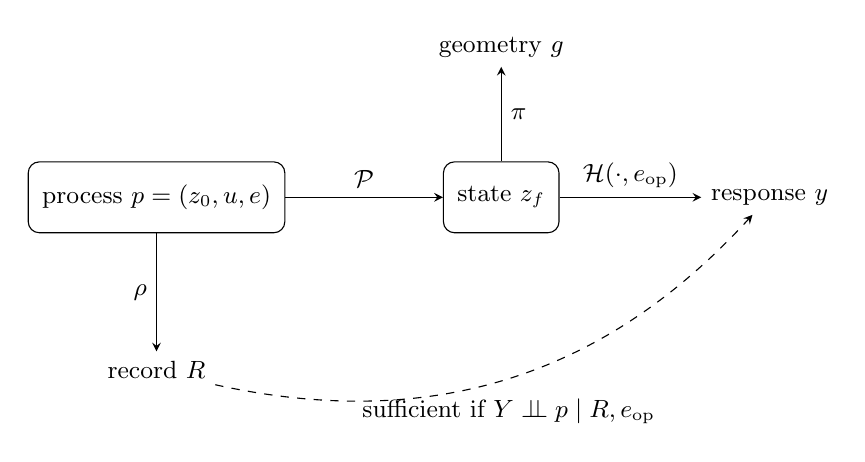
\begin{tikzpicture}[>=stealth, every node/.style={font=\small}, box/.style={draw, rounded corners, minimum height=0.9cm, inner sep=5pt}]
\node[box] (p) {process $p=(z_0,u,e)$};
\node[box, right=2.0cm of p] (z) {state $z_f$};
\node[right=1.8cm of z] (y) {response $y$};
\node[above=1.2cm of z] (g) {geometry $g$};
\node[below=1.5cm of p] (R) {record $R$};
\draw[->] (p) -- node[above] {$\mathcal{P}$} (z);
\draw[->] (z) -- node[above] {$\mathcal{H}(\cdot,e_{\mathrm{op}})$} (y);
\draw[->] (z) -- node[right] {$\pi$} (g);
\draw[->] (p) -- node[left] {$\rho$} (R);
\draw[->, dashed] (R) to[bend right=30] node[below=4pt, midway] {sufficient if $Y\perp\!\!\!\perp p\mid R,e_{\mathrm{op}}$} (y);
\end{tikzpicture}
\caption{The pipeline from process to response. The geometry $g$ is a projection of the final structural state and is in general an insufficient record (Proposition~\ref{prop:nonid}); a record $R$ is sufficient when it carries all of the information in the process that bears on the response (Section~\ref{sec:suff}). The pipeline is shared by the material systems considered here, whereas the operator $\mathcal{F}$ inside $\mathcal{P}$ differs among melt growth, extrusion of ordered fluids, transport in porous media, and solution crystallization.}
\label{fig:pipeline}
\end{figure}

Sufficiency is always relative to a specified class of admissible processes and operating conditions. Let $\mathcal{Q}$ denote that class, including the ranges of process inputs, feedstocks, apparatus conditions, and operating environments over which the claim is intended to hold. Three domains should be distinguished, because they need not coincide: the domain $\mathcal{Q}$ over which sufficiency is claimed, the distribution over $\mathcal{Q}$ used to estimate predictive risk during model development, and the held-out conditions used to challenge the claim. A record that is sufficient on the distribution sampled during development need not remain sufficient throughout $\mathcal{Q}$. In particular, a record may predict response accurately within one alignment regime while omitting variables that become decisive near a switching boundary. The claimed domain must therefore be declared before validation, and the validation design must include held-out conditions at its boundaries, and not only randomly withheld observations from its interior. Predictive performance outside the declared domain is evidence about a possible extension of the claim, not evidence that the original claim was established there.

Passing such tests supports sufficiency at the stated resolution and does not prove conditional independence. Finite observations cannot exclude every omitted process variable or every distribution shift within a broad class. That limitation is not a defect of the program. It is the reason that the claim is stated with a domain, an operational tolerance, and a reproducible validation protocol, and it is the sense in which Proposition~\ref{prop:suff} is used: as a statement about what a sufficient record is, while the experiments assess whether a given record is sufficient enough, over a given domain, to be relied upon.

%--------------------------------------------------------------------
\section{Structural Propositions and Their Consequences}

\subsection{Order is not uniformity}

The success of metallic single-crystal growth and the demonstrated value of internal gradients appear opposed until two notions are separated. Order, in the sense used here, refers to the persistence of a symmetry or alignment, such as a common crystallographic orientation across a component or a common director across a printed filament. Uniformity refers to the spatial constancy of every property. A single crystal can have a spatially varying dislocation density, a graded precipitate distribution, and a nonuniform residual stress while being a single crystal in the sense of orientation. Order and uniformity are therefore logically independent, and manufacturing objectives that conflate them can be internally contradictory.

A schematic formulation of a manufacturing objective that respects this distinction is
\begin{equation}
\min_{u(\cdot)}\ \Bigl[\lambda_1\,D_{\mathrm{harm}}(z_f)+\lambda_2\,\Gamma_{\mathrm{fun}}(z_f)+\lambda_3\,C_{\mathrm{prod}}(u)\Bigr],
\label{eq:objective}
\end{equation}
where $D_{\mathrm{harm}}$ measures structural irregularities that degrade the intended function, $\Gamma_{\mathrm{fun}}$ measures deviation of the achieved response from the target, and $C_{\mathrm{prod}}$ measures the cost of production in energy, time, material, and equipment utilization. The essential point is that $D_{\mathrm{harm}}$ is not a functional of the total variation of $z_f$. It is a functional of those components of variation that the response operator $\Hmap$ is sensitive to in a harmful direction. Whether a given feature belongs in $D_{\mathrm{harm}}$ or in $\Gamma_{\mathrm{fun}}$ is an empirical question about $\Hmap$ and cannot be answered by examining the material for irregularity alone.

\begin{hypothesis}[Selective organization]
\label{hyp:selective}
For a metallic system grown by pulsed remelting, there exist process settings under which crystallographic continuity and a prescribed gradient of dislocation density or precipitate fraction can be established together, and the resulting specimens outperform both a polycrystalline control and a gradient-free single-crystal control on a defined combination of yield strength, elongation, and creep life.
\end{hypothesis}

The hypothesis is falsifiable in at least two distinct ways. It fails if no process window exists in which orientation continuity survives while a gradient is imposed, which would indicate that the two are coupled through the thermal history at a level that cannot be broken. It also fails if the combined state exists but confers no advantage over its simpler controls.

\subsection{Correction versus accumulation}

A process may be said to accumulate if each increment of material is added to the object without subsequent alteration of material that is already present. A process corrects if increments are followed by operations that reorganize recently deposited material in response to its state. The schematic discrete-time form is
\begin{equation}
z_{k+1}=\mathcal{C}\bigl(\mathcal{D}(z_k,u_k),\,v_k\bigr),
\end{equation}
where $\mathcal{D}$ is a deposition operator, $\mathcal{C}$ is a correction operator, and $v_k$ is the correction input. In pulsed remelting, $\mathcal{D}$ adds a layer and $\mathcal{C}$ partially remelts it and the substrate surface, allowing resolidification onto the underlying lattice \cite{liu2026}. The same abstract structure appears in annealing steps interleaved with deposition, in solvent vapor treatment of printed films, and in thermal cycling of printed polymers to reset order.

\begin{definition}[Contractive correction]
A correction operator $\mathcal{C}$ is contractive with respect to a disorder functional $D$ on a set $S$ of states if $D(\mathcal{C}(z,v))\le \kappa\,D(z)$ for some $\kappa<1$ and all $z\in S$.
\end{definition}

\begin{proposition}[Bounded steady-state disorder]
\label{prop:contraction}
Suppose deposition introduces additional disorder of at most $\delta$ per step, so that $D(\mathcal{D}(z,u))\le D(z)+\delta$, and suppose $\mathcal{C}$ is contractive with constant $\kappa<1$ on all states reached. Then $D(z_k)\le \kappa^k D(z_0)+\delta\,\kappa\,\dfrac{1-\kappa^k}{1-\kappa}$, and in particular $\limsup_k D(z_k)\le \dfrac{\kappa\,\delta}{1-\kappa}$.
\end{proposition}

\begin{proof}
By induction. The inequality holds for $k=0$ trivially. If it holds for $k$, then $D(z_{k+1})\le\kappa\bigl(D(z_k)+\delta\bigr)\le \kappa^{k+1}D(z_0)+\delta\,\kappa\,\dfrac{1-\kappa^{k}}{1-\kappa}\,\kappa+\kappa\delta$, and the final two terms combine to $\delta\,\kappa\,\dfrac{1-\kappa^{k+1}}{1-\kappa}$. The limit follows since $\kappa^k\to0$. \qedhere
\end{proof}

The proposition is a statement about a model and not a claim about any physical process. It nevertheless clarifies what experimental data would be needed to support the interpretation that pulsed remelting works by contractive correction. One would have to demonstrate that the disorder introduced per layer is bounded, that the pulse removes a stable fraction of existing disorder, and that the combination yields a plateau in measured misorientation as growth height increases rather than a steady accumulation. The model also exposes the possibility of failure. If the correction operator is contractive with respect to grain misorientation but expansive with respect to some other functional, such as residual stress or solute segregation, the corrected structure can be worse by another measure. The correction must be assessed against the complete objective, and physical self-correction is not global optimization.

The scalar formulation treats disorder as a single quantity, whereas a growing structure carries several, and the preceding remark that remelting may improve one while worsening another can be made precise. Let $\mathbf{D}(z)=(D_1(z),\ldots,D_m(z))$ collect nonnegative measures of misorientation, residual stress, solute segregation, and similar deviations, and suppose that one cycle of deposition and correction satisfies, componentwise,
\begin{equation}
\mathbf{D}_{k+1}\le K\,\mathbf{D}_k+\mathbf{b},
\label{eq:coupled}
\end{equation}
where $K$ is a nonnegative matrix whose diagonal entries describe the self-correction of each measure and whose off-diagonal entries describe the coupling by which depositing or correcting with respect to one measure feeds another, and $\mathbf{b}\ge 0$ describes the disorder introduced per cycle.

\begin{proposition}[Coupled bounded disorder]
\label{prop:coupled}
Let $\mathbf{D}_0\ge 0$ and let $\rho(K)$ denote the spectral radius of $K$. (i) If $\rho(K)<1$, then $\limsup_k \mathbf{D}_k\le (I-K)^{-1}\mathbf{b}$ componentwise. (ii) If $K$ is irreducible, $\rho(K)\ge 1$, and $\mathbf{b}>0$, then the recurrence taken with equality has iterates that grow without bound, so that no bound follows from the recurrence.
\end{proposition}

\begin{proof}
(i) Since $K$ is nonnegative it preserves componentwise inequalities, and induction gives $\mathbf{D}_k\le K^k\mathbf{D}_0+\sum_{j=0}^{k-1}K^j\mathbf{b}$. When $\rho(K)<1$ one has $K^k\to 0$ and $\sum_{j\ge 0}K^j=(I-K)^{-1}$. (ii) Let $\mathbf{u}>0$ be a left Perron vector of $K$, so that $\mathbf{u}^{\top}K=\rho(K)\mathbf{u}^{\top}$. With equality in the recurrence, $\mathbf{u}^{\top}\mathbf{D}_{k+1}=\rho(K)\,\mathbf{u}^{\top}\mathbf{D}_k+\mathbf{u}^{\top}\mathbf{b}\ge \mathbf{u}^{\top}\mathbf{D}_k+\mathbf{u}^{\top}\mathbf{b}$, so that $\mathbf{u}^{\top}\mathbf{D}_k\ge k\,\mathbf{u}^{\top}\mathbf{b}\to\infty$. \qedhere
\end{proof}

The scalar proposition is the case $m=1$. The vector form shows that every diagonal entry of $K$ can lie below one, so that each measure contracts when considered alone, while off-diagonal coupling is strong enough to push the spectral radius to one or above, in which case the linear comparison model no longer guarantees that the structure is jointly bounded. The spectral radius, and not the best-behaved diagonal entry, determines whether the corrected structure is stable. Estimating $K$ from layer-by-layer measurements of several deviation measures is accordingly a concrete experimental objective, taken up in Strand C. When the recurrence is an inequality and $\rho(K)\ge 1$, the actual iterates may still be bounded by mechanisms that the linear recurrence does not represent, which is why the question of whether the physical coupling is strong enough to matter is empirical and is posed as Hypothesis~\ref{hyp:coupled}.

\subsection{Serial transport and diminishing return}

Transport across scales can be idealized as a series of resistances. If $R_{\mathrm{macro}}$, $R_{\mathrm{micro}}$, and $R_{\mathrm{nano}}$ denote resistances to bulk flow through channels, diffusion through finer porosity, and sorption or reaction at molecular sites, the idealized total is
\begin{equation}
R_{\mathrm{tot}}=R_{\mathrm{macro}}+R_{\mathrm{micro}}+R_{\mathrm{nano}},
\end{equation}
and the flux under a fixed driving potential $\Delta P$ is $J=\Delta P/R_{\mathrm{tot}}$. The actual systems involve coupled diffusion, adsorption, heat transport, and convection and do not reduce strictly to a linear network, so this is a conceptual approximation.

\begin{proposition}[Bounded benefit of single-scale improvement]
\label{prop:series}
In the series model, with all $R_j\ge0$ and with $R_{\mathrm{tot}}-R_i>0$, so that the remaining resistances have a strictly positive sum, the maximum relative improvement of flux achievable by reducing a single resistance $R_i$ to zero is $\dfrac{R_i}{R_{\mathrm{tot}}-R_i}$, and the elasticity of flux with respect to $R_i$ is $\partial\ln J/\partial\ln R_i=-R_i/R_{\mathrm{tot}}$, so that the proportional benefit of improving one scale is set by the share of the total resistance that the scale carries.
\end{proposition}

\begin{proof}
Setting $R_i\to0$ gives $J'=\Delta P/(R_{\mathrm{tot}}-R_i)$, and $J'/J-1=R_i/(R_{\mathrm{tot}}-R_i)$. For the elasticity, $\ln J=\ln\Delta P-\ln R_{\mathrm{tot}}$, so that $\partial\ln J/\partial R_i=-1/R_{\mathrm{tot}}$, and multiplication by $R_i$ gives the result. If $R_i$ were the only positive resistance, eliminating it would leave zero total resistance and an unbounded idealized flux, which is why the positivity of the remainder is assumed. \qedhere
\end{proof}

The proposition provides a precise form of the qualitative statement that matching of scales matters more than excellence at any one of them. The absolute derivative $\partial J/\partial R_i=-\Delta P/R_{\mathrm{tot}}^2$ is the same for every scale and therefore cannot rank them, since an equal absolute reduction of any resistance buys the same gain in flux, whereas the elasticity is dimensionless and ranks the scales by their share of the total, which is the relevant guide when interventions achieve proportional and not absolute reductions. It also suggests an experimental diagnostic. If measured performance is insensitive to a large change in a resistance that has been designed to improve, then another resistance is limiting, and effort is better directed there. The diminishing increment observed when a fourth hierarchical order was compared to a third \cite{bai2026} is of this kind, although the proposition alone does not establish that the series model describes that system, and the authors' own explanation involves limited space and diffusion depth in the finer channels together with printability. An additional possibility is that higher-order hierarchy reduces the effective volume of active material or increases mechanical fragility, so that a competing cost rises as the transport resistance falls. A genuine optimum then exists in the interior of the design space, as the reported porosity trade-off between gravimetric and volumetric kinetics already suggests, and the proper task is to find it with measurements that separate the competing effects.

\subsection{The inverse problem and its ill-posedness}

The distinguishing ambition of the research direction is to invert the traditional order of design. Given a target response $y^\ast$, one seeks the process inputs that yield it:
\begin{equation}
u^\ast=\arg\min_{u(\cdot)}\ \Bigl\{\bigl\|\Hmap\bigl(\Pmap[z_0,u,e],e_{\mathrm{op}}\bigr)-y^\ast\bigr\|_W^2+\lambda\,C[u]\Bigr\},
\label{eq:inverse}
\end{equation}
where $W$ weights the components of the response and $C$ penalizes cost. The formulation is the author's synthesis and is not a model claimed by any of the experimental studies discussed.

Inverse problems of this form are often ill-posed in the sense of Hadamard. Existence may fail if the target lies outside the set of achievable states, uniqueness fails whenever the functional equivalence class of the target contains more than one process, and stability fails if small changes in measured response correspond to large changes in the inferred inputs. All three modes are physically plausible here. Existence fails for responses that require incompatible states, such as a printed liquid-crystalline filament with an actuation strain exceeding what its molecular order can supply. Non-uniqueness is the generic situation, since the same final state can often be reached by many thermal schedules, and different states can produce similar responses. Instability is most acute near phase or alignment boundaries, where infinitesimal changes in conditions switch the state qualitatively. The practical consequence is that inversion requires regularization that encodes manufacturability and cost, and that the structure of the set of solutions should be reported rather than hidden behind a single optimum. For practical inversion the relevant question is less whether the problem is ill-posed in principle than whether the regularized solution is stable enough to be useful, and that is an empirical matter answered by the replicate and held-out experiments of the strands below.

\subsection{Phase boundaries as the informative region of process space}

A recurring feature of the systems above is the existence of discontinuous or sharply nonlinear transitions in process space: the switch between parallel and perpendicular alignment in smectic elastomers, the onset of equiaxed grain formation in metal deposition, the transition from supersaturated deposition to nucleation-dominated crystallization in antisolvent spraying. Experimental effort spread uniformly over process space oversamples regions where the response varies smoothly and undersamples the regions where the underlying physics changes. Hypothesis-driven programs should therefore weight their sampling toward boundaries, and the models they produce should be evaluated on held-out conditions near and across boundaries. Interpolation accuracy within the smooth interior does not establish the ability to predict switching.

%--------------------------------------------------------------------
\section{Research Program}

The research program is organized into seven strands. They are not sequential stages. Strands A to D concern four material classes and each can proceed independently. Strand E concerns the cross-cutting measurement and record infrastructure. Strand F concerns integration of established capabilities into devices. Strand G concerns closed-loop experimental design. The strands are described with enough specificity that the hypotheses they test could be written as protocols, and each contains an explicit statement of what would count as failure. Each strand also states which proposition or hypothesis of the formal development it probes, and Table~\ref{tab:hyp} collects the hypotheses with their falsification conditions.

Two objects are designated as candidates for transfer across material systems, so that the claim of a single program acquires an operational test. The first is the resistance decomposition, in which the total resistance of a transport or conversion chain is measured as a sum of independently measured contributions and the elasticity $R_i/R_{\mathrm{tot}}$ of each contribution is used to rank interventions. It applies in a literal sense to the sorbent monoliths of Strand B and, once channel resistance is separated from contact and domain-boundary resistance by length-dependent measurements, to the transistors of Strand D, and these two strands carry the first-phase commitment. Its application to the metallic strand, where the relevant chain would run through melt pool, substrate, and part, is exploratory and is not assumed to hold. The second candidate is the sufficiency construction of Section~\ref{sec:suff}, which is tested in Strands A and D, where specimens are inexpensive, and in Strand E, where transfer between laboratories is examined. Transfer is judged by two criteria fixed in advance, formalized as Hypotheses~\ref{hyp:transfer} and~\ref{hyp:suftransfer}: that a decomposition protocol developed in one strand ranks the effects of a set of interventions correctly in the other, at a rate exceeding chance by a stated margin, with the ranking statistic, tie rule, and decision margin held fixed and only the resistance measurements changed, and that a compact record found sufficient in one system by a given selection procedure is found sufficient in the other at a comparable margin. If neither criterion is met at the end of the first phase, the program should be regarded as a set of separate programs sharing a record format.

\subsection{Strand A: Process-to-structure maps for responsive polymer networks}

\subsubsection*{Rationale}

Liquid-crystalline elastomers printed from smectic inks offer a favorable setting for studying process-dependent function because the key structural variable, the director field, is accessible to polarized optical and X-ray scattering measurements, and the functional variable, actuation strain, is measurable by simple imaging. The existence of a switch between two alignment regimes under variation of print temperature and shear, attributed to the preservation or collapse of smectic layers near a critical shear rate, provides a built-in boundary to study \cite{lee2026}.

\subsubsection*{Objective}

The objective is to establish a predictive and experimentally validated relation of the form
\begin{equation}
\bigl(\dot\gamma,\ T_p,\ v,\ d_n,\ h\bigr)\ \longmapsto\ \bigl(\mathbf{n}(\mathbf{x}),\ S,\ \epsilon_{\mathrm{act}}\bigr),
\end{equation}
where $\dot\gamma$ is the shear rate at the nozzle, $T_p$ the print temperature, $v$ the printing speed, $d_n$ the nozzle diameter, $h$ the layer height, $\mathbf{n}$ the director field, $S$ the scalar order parameter, and $\epsilon_{\mathrm{act}}$ the actuation strain on thermal cycling through the transition.

\subsubsection*{Experimental design}

A factorial design over $\dot\gamma$ and $T_p$ is used to locate the alignment boundary, followed by adaptive refinement concentrated near the boundary. For each condition, filaments and thin sheets are printed and characterized by polarized optical microscopy, small-angle and wide-angle X-ray scattering where available, and by differential scanning calorimetry. Actuation is measured in free-standing specimens under controlled thermal cycles with video extensometry. A subset of specimens is subjected to extended cycling to establish whether the printed state is stable or drifts toward a relaxed order.

Models are trained on a fraction of the conditions, and evaluation is conducted on three held-out sets: interior conditions, boundary conditions, and conditions that vary a parameter, such as nozzle diameter, that was held fixed during training. The last set is the most informative, because it tests whether the model has captured a mechanism or merely a response surface on a single apparatus.

\begin{hypothesis}[Shear-temperature collapse]
\label{hyp:collapse}
The alignment regime of printed smectic elastomers is determined by a small number of dimensionless groups, in particular a Weissenberg-like number formed from shear rate and a layer-relaxation time that depends on temperature and on proximity to the transition, such that data collected on different nozzle diameters and speeds collapse onto a single boundary in the reduced variables.
\end{hypothesis}

The hypothesis fails if boundaries measured with different nozzles do not collapse after rescaling, which would indicate that wall slip, thermal gradients across the nozzle, or ink preconditioning contribute in ways that the proposed groups do not capture.

\subsubsection*{Deliverables and measures of success}

A successful strand produces a boundary model validated to within a stated tolerance on held-out nozzle geometries, a map of actuation strain across the process space with uncertainty, a quantified bound on strain drift over thermal cycling, and a set of programmed demonstrators in which regions of one sign of response are co-printed with regions of the opposite sign within a single object. The final item is the most direct test of whether conditions can be changed along a print path to write a spatial program into a continuous material. The strand probes Proposition~\ref{prop:nonid} in a system in which the same toolpath is known to give opposite responses, and it supplies the data for Hypothesis~\ref{hyp:compact}.

\subsection{Strand B: Structure-to-function optimization of hierarchical transport architectures}

\subsubsection*{Rationale}

Hierarchically porous sorbents embody the multiscale constraint of Proposition~\ref{prop:series} in a form that can be tested directly. The reported selection of a third-order hierarchy over a fourth-order one, on grounds of smaller marginal kinetic gain and printability \cite{bai2026}, together with the reported trade-off between porosity and volumetric kinetics, suggests that an interior optimum exists, and the open questions are what determines its location and how general it is across sorbent chemistries, climates, and cycling regimes.

\subsubsection*{Objective}

The objective is to determine how channel hierarchy, porosity, tortuosity, and monolith thickness influence kinetics and net yield, and to separate the contribution of hierarchy from that of other differences between printed and packed configurations.

\subsubsection*{Experimental design}

Because a more elaborate channel hierarchy displaces sorbent and alters accessible surface area, external dimensions and active sorbent mass cannot in general be held fixed together, and the design therefore reports two comparisons separately and does not attempt to remove the trade-off by matching. In the volumetric comparison, hierarchical monoliths of orders zero to four are printed from the same sorbent formulation inside a common external envelope, with airflow, humidity, and regeneration conditions fixed, and performance is expressed per unit external volume. In the gravimetric comparison the active sorbent mass is held fixed, the external volume is allowed to vary, and performance is expressed per unit mass of sorbent. Each comparison includes randomly packed material and a simple parallel-channel monolith as references. The difference between the two sets of results exposes directly the trade-off between porosity and volumetric kinetics that the source work identifies as favouring medium porosity \cite{bai2026}. Sorption and desorption kinetics are recorded at several humidity and temperature conditions, cycling over several hundred cycles establishes durability, and post-cycling imaging tests whether channels or pore networks degrade.

The performance measure is neither water yield in isolation nor an instantaneous rate. Writing $m(n)$ for the water delivered in cycle $n$, $E_{\mathrm{cycle}}(n)$ for the energy consumed in that cycle, and $E_{\mathrm{mfg}}$ for the embodied manufacturing energy, the lifetime-integrated energy-normalized yield is
\begin{equation}
\eta_w^{\mathrm{life}}=\frac{\sum_{n=1}^{N_{\mathrm{life}}}m(n)}{E_{\mathrm{mfg}}+\sum_{n=1}^{N_{\mathrm{life}}}E_{\mathrm{cycle}}(n)},
\end{equation}
where $N_{\mathrm{life}}$ is fixed by a stated end-of-life criterion, such as the cycle at which delivered water per cycle falls below a stated fraction of its initial value. Without the lifetime term, an architecture that is optimal at first use and degrades quickly cannot be distinguished from one with identical initial performance that endures. The quantity is reported together with production rate per unit volume, mass-specific yield, and an estimate of material and manufacturing cost.

\begin{hypothesis}[Interior optimum in hierarchy]
\label{hyp:interior}
At fixed humidity and regeneration energy, $\eta_w^{\mathrm{life}}$ is a non-monotonic function of channel order, with a maximum at an intermediate order.
\end{hypothesis}

\begin{hypothesis}[Humidity dependence of the optimum]
\label{hyp:humidity}
The channel order that maximizes $\eta_w^{\mathrm{life}}$ varies with ambient humidity, and the direction of the variation is the one predicted by which resistance dominates at each humidity in the independent decomposition described below.
\end{hypothesis}

Two physical arguments predict opposite directions of shift. If vapor transport through the channel network is the limiting step at low humidity, where the driving potential is small, then architectures that lower the macroscale resistance are rewarded and the optimum moves toward higher order as humidity falls. If instead intrinsic sorption kinetics dominate at low humidity, because the sorbent then operates further from saturation and takes up water slowly whatever the access, then added hierarchy costs sorbent volume without relieving the limiting step, and the optimum is insensitive to humidity or moves toward lower order. The experiment discriminates between the two accounts, and either outcome is informative. The second hypothesis is not established by the source work and is conditional on the decomposition identifying the limiting step. It fails if the observed direction of shift contradicts the direction predicted from the measured elasticities, which would count against the adequacy of the series model under the tested conditions, although inaccurate resistance measurements or an incomplete decomposition could produce the same outcome.

\subsubsection*{Resistance decomposition}

To test the series interpretation, independent measurements of the resistances are required. Bulk permeability of the channel network can be measured with pressure-drop experiments on non-sorbing replicas of the same geometry. Effective diffusivity in the finer porosity can be measured on thin samples whose thickness is below the channel scale. Intrinsic sorption kinetics can be measured on powder samples under conditions in which transport is not limiting. Comparison of the sum of independently measured resistances with the observed total tests whether the series model is adequate, and the residual quantifies the coupling that it neglects. The resulting shares $R_i/R_{\mathrm{tot}}$ are the elasticities of Proposition~\ref{prop:series} and supply an a priori ranking of the scale that should be improved next, a ranking that can then be tested by intervention. The strand thereby probes Proposition~\ref{prop:series} and supplies the sorbent half of Hypothesis~\ref{hyp:transfer}.

\subsubsection*{Generalization}

The same design transfers to catalytic monoliths, electrode architectures, thermal exchangers, and tissue scaffolds, because each involves coordinated transport at several scales and a conflict between surface area and permeability. A secondary objective of the strand is to identify whether the functional form of the optimum is shared across such systems when expressed in dimensionless variables, which would support the proposal that multiscale design has a common structure.

\subsection{Strand C: Controlled elimination and retention of structural variation in metals}

\subsubsection*{Rationale}

The coexistence of single-crystal continuity with beneficial gradients is the point at which two recent lines of work meet \cite{liu2026,guo2025}. The authors of the single-crystal work already attribute the creep behavior of the titanium alloy to a combination of grain-boundary elimination and an additive-manufacturing-induced hierarchical alpha and beta architecture \cite{liu2026}, which is itself an engineered internal heterogeneity, so that the question is not whether structured heterogeneity coexists with orientation continuity but how far it can be controlled independently. It is also the point at which the largest uncertainty lies, because the thermal conditions that suppress competing grains alter dislocation generation, precipitation, and segregation. Whether these effects can be decoupled is an empirical question that cannot be settled from the existing evidence.

\subsubsection*{Objective}

The objective is to map the relations among thermal history, crystallographic continuity, internal gradients, and mechanical response in additively manufactured single crystals, and to identify process windows in which continuity is maintained while specified gradients are imposed.

\subsubsection*{Experimental design}

Specimens of matched macroscopic geometry and crystallographic orientation are produced under a designed set of thermal schedules that vary pulse energy, pulse duration, interlayer dwell time, and the ratio of deposition to remelting energy, with the published cycle of a pulse of about half a second followed by a resolidification interval of about nine and a half seconds serving as the reference condition \cite{rohrer2026}. Each specimen is characterized by electron backscatter diffraction for orientation and misorientation, by electron microscopy and, where available, atom probe or spectroscopic methods for precipitates and composition, by X-ray or neutron diffraction for residual stress, and by line profiling of hardness as a proxy for dislocation density. Mechanical testing includes tensile tests with full-field strain measurement, creep tests at relevant temperatures, and, for the titanium-based system, examination of the variant structure that develops on cooling \cite{rohrer2026}.

The principal analysis is a decomposition of the property response into contributions from orientation continuity, interface density, and gradient magnitude, using the designed variation to separate them. Interface density includes interfaces generated by solid-state transformation, so the analysis distinguishes between growth-temperature single-crystallinity and service-temperature interface content.

\begin{hypothesis}[Separable control]
\label{hyp:separable}
There exists a process window in which gradient magnitude, measured as the spatial standard deviation of a defined local hardness or dislocation density proxy over a specified length, can be varied by at least a factor of two without introducing misoriented grains above a stated area fraction.
\end{hypothesis}

\begin{hypothesis}[Functional gradient advantage]
\label{hyp:gradientadv}
Within that window, a specimen with an optimized gradient exhibits a larger product of yield strength and uniform elongation than a gradient-free single crystal of the same composition and orientation, in a loading mode matched to the gradient.
\end{hypothesis}

The matching of gradient to loading is a design requirement, not an excuse. A gradient designed for tension may be irrelevant to fatigue or creep, and the claim of advantage is therefore restricted to the mode specified in advance. The strand reports results for all loading modes tested, including those in which no advantage is found.

\begin{hypothesis}[Coupled correction]
\label{hyp:coupled}
In pulsed remelting, the diagonal entry of the coupling matrix of Equation~\eqref{eq:coupled} for misorientation lies below one, while the coupling from the remelting step into residual stress is large enough that the estimated spectral radius approaches or exceeds one at larger section sizes, so that the accessible diameter is limited by accumulating residual stress and not by loss of orientation control.
\end{hypothesis}

The commentary reports that the crystal diameter is currently limited to between 6 and 20 millimeters without attributing the limit to a mechanism \cite{rohrer2026}, and the hypothesis offers one candidate that can be tested by measuring misorientation and residual stress as functions of height and diameter and fitting $K$. It fails if misorientation rises with diameter while residual stress remains small, which would place the limit in orientation control, or if neither measure shows accumulation, which would point to a limit of melt-pool or mechanical stability instead. It also fails if the estimated spectral radius stays well below one at the largest sections studied, even when residual stress increases, since the coupled mechanism would then not be the one that sets the limit.

Two identification problems are stated here because they determine what the measurements can support. The first is that the recurrence of Proposition~\ref{prop:coupled} is an inequality, and many nonnegative matrices satisfy the same inequality when the sampled states cover only a narrow range. A matrix obtained by regressing one layer's deviation vector on the previous one estimates an average transition model, which is a different object from a matrix that validates a componentwise upper bound. The strand accordingly distinguishes the two tasks. Estimation of the average model uses perturbations that vary the deviation components independently, for example by changing remelting parameters and section size separately, and reports uncertainty bounds on the entries of $K$ and on its spectral radius. Validation of the upper-bound model checks on held-out layers and sections that the fitted bound is not exceeded. The second is that the connection between the spectral radius and the reported diameter limit is a hypothesis, which the measurements may or may not support, and it is not a deduction from the proposition. The strand thereby probes Propositions~\ref{prop:contraction} and~\ref{prop:coupled} and the separation of order from uniformity stated in Hypothesis~\ref{hyp:selective}.

\subsubsection*{Complications specific to the metallic case}

Several complications distinguish this strand from the others in expense and in analytic difficulty. Process control requires thermal imaging and current monitoring at high temporal resolution, and the relevant length scales span the melt pool to the full component. Characterization is destructive for most techniques, and a given specimen can therefore be examined in only a few ways, which makes the design of the sampling plan a first-order concern. The coupling among melting, solidification, solid-state transformation, and thermal stress produces strongly nonlinear mappings, and the inverse problem of Equation~\eqref{eq:inverse} is correspondingly harder than for polymers. For these reasons the strand is likely to proceed more slowly than the others, and its most realistic early output is a structured dataset of thermal histories with matched characterization, which would itself be valuable for the development of reduced-order process models.

\subsection{Strand D: Functional equivalence in organic electronic materials}

\subsubsection*{Rationale}

The coexistence of polycrystalline films with near-single-crystal performance, and of directly formed single crystals with the same performance, supplies a clean test of the claim that function does not determine structure uniquely \cite{niazi2015,rigas2016}. It is also an arena in which the question of which structural features matter has practical consequences, since the cheaper process is preferred if the performance is equivalent. The reported dependence of blend performance on the identity of the insulating polymer, at nearly equal thermodynamic driving force for phase separation \cite{niazi2015}, shows that the relevant descriptors include morphology realized during coating and cannot be read from composition.

\subsubsection*{Objective}

The objective is to determine which structural descriptors predict device-level performance across processing routes, and in particular whether a small set of descriptors, such as the fraction of boundaries that are transport-blocking, the mean orientation of the packing direction relative to the channel, and the vertical composition profile in blends, collapses data from polycrystalline and single-crystal devices onto a common relation.

\subsubsection*{Experimental design}

Devices are fabricated by blade coating of blends and by spray-based antisolvent crystallization, over a range of molecular weights, blend ratios, deposition speeds, and substrate treatments, and with channel dimensions varied relative to crystal or domain size. Each device is characterized electrically, and its active layer is characterized structurally by grazing-incidence X-ray diffraction, polarized microscopy, and, where destructive analysis is acceptable, vertical composition profiling. A regression is fitted of electrical performance against structural descriptors, with route as a categorical variable.

\begin{hypothesis}[Descriptor sufficiency]
\label{hyp:descriptor}
After conditioning on the structural descriptors, the differences between deposition routes in mobility, threshold voltage, and subthreshold swing lie within equivalence margins fixed in advance.
\end{hypothesis}

Failure to detect a route effect is not evidence that the effect is absent, so the hypothesis is assessed by an equivalence test, such as two one-sided tests against margins set from device-to-device variability, and not by a null-significance test. It fails if the confidence interval for the route difference extends beyond a margin. The hypothesis concerns predictive equivalence and not causal mediation. Descriptors measured after fabrication lie downstream of the deposition route, and conditioning on them can introduce selection effects or hide pathways that run through unmeasured variables, so that a finding of equivalence does not show that the route has no causal influence on device performance. Causal mediation is reserved for experiments designed to identify it, for example by manipulating descriptors independently of route, and it is not claimed here. The outcome in which route retains predictive power is arguably the more interesting one, because it may point to an unmeasured variable and thereby extend the state description.

Devices are in addition fabricated with a range of channel lengths, so that the transfer-length method separates contact resistance from channel resistance, and where domain size is varied the channel resistance is further separated into bulk-film and domain-boundary contributions. The total resistance is thereby decomposed in the same series form as in Strand B, and the elasticity ranking is compared with the measured effect of interventions such as contact treatment, annealing, and change of blend ratio.

\begin{hypothesis}[Transfer of the decomposition]
\label{hyp:transfer}
A resistance-decomposition protocol developed in Strand B, applied in Strand D with the ranking statistic, the tie rule, and the decision margin held fixed, and with only the measurements of the resistances themselves changed, ranks the effect of a set of interventions on device performance correctly at a rate exceeding chance by a margin fixed in advance, and the converse holds for a protocol developed in Strand D and applied to the sorbent monoliths.
\end{hypothesis}

The protocol fixes three things before data are collected. The ranking statistic is the elasticity $R_i/R_{\mathrm{tot}}$ of each contribution with an interval estimate, and the set of interventions is declared in advance. Correctness is scored pairwise, as agreement between the predicted order of two interventions and the order of their measured effects, with chance at one half. Two interventions whose elasticity intervals overlap are declared tied, are excluded from the numerator and the denominator of the ranking rate, and are counted separately, and a protocol that leaves most pairs tied is reported as uninformative and not as a success.

Strand D probes the claim that the mapping from function back to structure is not one to one, which is the empirical counterpart of Proposition~\ref{prop:nonid}, and it supplies the transistor half of Hypothesis~\ref{hyp:transfer}.

\subsection{Strand E: Process-state records, measurement standards, and shared infrastructure}

\subsubsection*{Rationale}

The cumulative character of the other strands depends on the quality of the records in which their data are kept. If one laboratory reports print temperature as a set point and another as a measured nozzle temperature, if thermal histories are stored as images without time stamps, or if characterization conditions are omitted, then data cannot be pooled and models cannot be tested outside the laboratory in which they were trained. The existing literature is typically rich in headline results and poor in the machine-readable detail needed to reuse them.

\subsubsection*{Objective}

The objective is a record format and a set of reporting norms for process-dependent materials work. A record contains the specification of the feedstock and substrate, the full process trajectory $u(\cdot)$ at the temporal resolution of the controller, the measured environmental history $e(\cdot)$, in-situ monitoring signals with calibration metadata, post-process characterization with instrument settings, functional test protocols with environmental conditions, and the identity and version of any model used to generate or select the conditions.

\subsubsection*{Components}

Four components are envisaged. The first is a schema for process trajectories that is independent of machine vendor, in which each controllable input is recorded with units, sampling rate, and a declaration of whether it is a commanded or measured quantity. The second is a catalogue of structural descriptors with defined measurement procedures, so that a statement such as misorientation fraction or order parameter has a unique operational meaning. The third is a protocol for reporting uncertainty, including repeat specimens, between-batch variation, and the rate of specimens excluded from analysis and the reasons for exclusion. The fourth is a registry of null and negative results, in which experiments that did not produce the expected structure are recorded with the same detail as those that did.

The registry deserves particular emphasis, because the boundary regions of process space are precisely where failures cluster, and published literature systematically under-represents them. A model trained only on successful conditions will overestimate the extent of the region in which the process works.

\begin{hypothesis}[Record transfer]
\label{hyp:record}
A model trained on process records from one laboratory predicts the structure and response of specimens fabricated in a second laboratory with comparable equipment with lower error when trained on measured process variables than when trained on commanded settings alone, by at least a margin fixed in advance.
\end{hypothesis}

This hypothesis can be tested by sharing a common ink, feedstock, or alloy batch between laboratories and comparing predictions made from commanded settings against predictions made from measured settings. If the improvement is smaller than the margin, the added burden of recording measured variables is unjustified for that system. A positive result shows that measured variables help and does not show that no other recording strategy could do as well, which is why the next hypothesis concerns the compactness of the record.

\begin{hypothesis}[Compact sufficient records]
\label{hyp:compact}
For the alignment-switching system of Strand A, a record consisting of a small number of measured variables, such as nozzle temperature, nozzle shear rate, and thermal dwell, is $\delta$-sufficient for actuation strain relative to the full set of logged variables, both on held-out conditions and on specimens fabricated in a second laboratory.
\end{hypothesis}

The process class $\mathcal{Q}$, the law $\mu$ under which processes are sampled, the minimum boundary margin, and the held-out validation regions are fixed before model fitting, and the validation regions include a resampling that weights the boundary more heavily than the development law does, so that sufficiency under $\mu$ is not mistaken for sufficiency under other sampling laws, and failure to meet the predictive-risk tolerance in any pre-specified validation region rejects the sufficiency claim over the full declared class, even if average risk remains low. The hypothesis also fails if $\delta$-sufficiency holds only within the originating laboratory, which would indicate that the compact record encodes apparatus-specific information and that the transferable record is larger. It is the central empirical test of the sufficiency construction, because it asks whether manufacturing history can be compressed into a representation that survives a change of apparatus.

\begin{hypothesis}[Sufficiency transfer]
\label{hyp:suftransfer}
A record-selection procedure that yields a $\delta$-sufficient compact record for actuation strain in Strand A, applied to mobility, threshold voltage, and subthreshold swing in Strand D with the feature-selection algorithm, model-selection criterion, validation protocol, and risk-normalization rule held fixed, and with only material-specific measurement transformations permitted, yields a compact record that is $\delta'$-sufficient for those device metrics, with $\delta'$ fixed in advance.
\end{hypothesis}

The hypothesis makes the sufficiency construction a cross-material claim and not a single-system demonstration. Material-specific transformations of the raw measurements are not counted as redesign, because the two systems differ in variables, units, sampling rates, and measurement error, and no procedure can accept literally identical inputs. The tolerances $\delta$ and $\delta'$ are expressed as excess risk relative to the risk of a predictor that ignores the record, so that actuation strain and mobility are compared on a common normalized scale, and the normalization is fixed before fitting. The hypothesis is deliberately posed across systems whose records differ in dimensionality, a low-dimensional and inexpensive one and a higher-dimensional and costly one, and it fails if the selection procedure must be redesigned for the second system, in which case sufficiency is a property of particular systems and not of the construction. Strand E thereby probes Proposition~\ref{prop:suff} and the transfer claim at the head of the program.

\subsection{Strand F: Functional integration of established capabilities}

\subsubsection*{Rationale}

The individual capabilities described above have been demonstrated separately. Their combination in devices would be significant but is not guaranteed to be feasible, since compatibility of materials, processing temperatures, and operating environments is not assured. The strand is accordingly framed as a set of feasibility studies with explicit go and no-go criteria, and not as a deliverable assumed to succeed. Each integration is stated together with the proposition or hypothesis it probes, and where an integration tests engineering viability only, that is said.

\subsubsection*{Programmable fluidic and reaction systems}

Printed reaction vessels in which the geometry influences product distribution \cite{symes2012} can be combined with responsive polymer elements \cite{vanoosten2009,lee2026} to produce valves, mixers, or constrictions that change state in response to temperature or light. The scientific question is whether dynamic modification of geometry within a reaction produces control of selectivity not available with a fixed geometry. A direct test is to compare a reaction carried out in a vessel whose mixing element is actuated during the reaction against the same reaction in vessels fixed in each of the actuator's two states. Advantage in selectivity or conversion attributable to the dynamics, and not to either static state, would indicate that time-varying geometry is a genuine experimental degree of freedom. The principal risks are chemical compatibility of the polymer with solvents and reagents, swelling, and thermal limits of the elastomer. This integration would test whether the sufficiency claim of Section~\ref{sec:suff} extends to records that include time-varying geometry, since the history of the actuator state becomes part of the process record.

\subsubsection*{Adaptive sorption structures}

Responsive elements might regulate airflow or thermal contact in hierarchical sorbent monoliths, for instance by opening channels during sorption and closing them during desorption to reduce parasitic heat loss. The decisive test is net benefit after accounting for actuation energy, mechanical reliability under cycling, and added complexity. A design in which the actuator consumes more than it saves fails the test regardless of how elegant the mechanism is. The integration tests the resistance decomposition of Proposition~\ref{prop:series} in a setting in which one resistance is made time-varying, and it is otherwise a test of engineering viability.

\subsubsection*{Functionally graded structural components}

If Strand C establishes a window of separable control, graded single-crystal components in which different regions are tuned for strength, ductility, or creep resistance become possible. An example would be a blade or lattice member in which the root has a gradient optimized for fatigue and the tip a gradient optimized for creep, within a single crystal that avoids grain boundaries as sites of failure. The integration challenge is precision of thermal control at the length scale of the gradient, and the strand's initial aim is a demonstration on a simple geometry before any claim about complex parts. The integration tests Hypotheses~\ref{hyp:separable} and~\ref{hyp:gradientadv} at the scale of a component, in which orientation continuity and a patterned gradient must hold together.

\subsubsection*{Criteria for integration}

For each integration the program specifies in advance the minimum improvement over the best non-integrated baseline that would count as success, the measurements by which it will be determined, and the conditions under which the project will be abandoned. The practice of specifying abandonment criteria before results are known is a deliberate protection against the tendency of integration projects to accumulate justifications for continuing after the evidence has turned against them.

\subsection{Strand G: Closed-loop experimental design}

\subsubsection*{Rationale}

The process spaces involved are high-dimensional, experiments are costly, and the relationships of interest are nonlinear and bounded by sharp transitions. These are the conditions under which sequential experimental design offers the largest advantage over fixed grids. A system that selects its next experiment on the basis of what has been learned can allocate effort to the boundaries and to the regions of greatest uncertainty.

\subsubsection*{Formulation}

The next set of process parameters is chosen by
\begin{equation}
u_{k+1}=\arg\max_{u\in\mathcal{U}}\ \Bigl[\E\bigl[J(u)\mid\mathcal{D}_k\bigr]+\beta\,I(u\mid\mathcal{D}_k)-\lambda\,C(u)\Bigr],
\end{equation}
where $\mathcal{D}_k$ is the data collected up to step $k$, $J$ is the uncertain functional performance, whose posterior mean enters the rule, $I$ is the expected information gain about the process-structure and structure-function relations, and $C$ is the cost of the experiment. The weight $\beta$ trades exploitation of the current best against exploration that reduces uncertainty. The information-gain term is a device of experimental design and carries no commitment to an information-theoretic definition of sufficiency, which is stated in terms of conditional laws and predictive risk. The framework is a proposal for experimental design, not a procedure demonstrated in the studies discussed here.

\subsubsection*{Safeguards}

Closed-loop optimization can fail in characteristic ways, and the program specifies safeguards against each. A surrogate model that is optimized against can be exploited, in the sense that the optimizer finds conditions at which the model's predictions are inaccurate and favorable. The safeguard is to reserve independent validation specimens that were never used in model fitting or in acquisition, and to report performance on those specimens alone as the evidence of improvement. A second failure is drift of the apparatus, as nozzles wear, feedstock lots change, and ambient conditions vary seasonally, which creates spurious structure in the data. The safeguard is periodic repetition of reference conditions, with the control data used to detect and model drift. A third is the reduction of a multi-objective problem to a scalar in a way that hides trade-offs. The safeguard is to maintain and report the Pareto set of achieved performances and not only the best scalar value.

\begin{hypothesis}[Efficiency of boundary-weighted acquisition]
\label{hyp:acq}
For the alignment-switching system of Strand A, an acquisition rule that includes the information term localizes the alignment boundary to a specified precision using at most half the experiments required by a space-filling design of equal final precision.
\end{hypothesis}

This hypothesis is quantitative and cheap to test, since Strand A already generates the required data, and it can be evaluated retrospectively on existing measurements before being tested prospectively. The strand thereby probes the inverse problem of Equation~\eqref{eq:inverse}, in particular whether weighting acquisition toward boundaries makes the inversion stable enough to be useful.


\subsection{Summary of hypotheses and falsification conditions}

\begin{small}
\setlength{\tabcolsep}{3pt}
\begin{longtable}{@{}p{1.2cm}p{4.1cm}p{4.3cm}p{3.7cm}@{}}
\caption{The hypotheses of the program, with the strand that carries each, the condition under which it would be rejected, and the primary endpoint on which the decision rests.}\label{tab:hyp}\\
\toprule
No. & Claim & Rejected if & Primary endpoint \\
\midrule
\endfirsthead
\toprule
No. & Claim & Rejected if & Primary endpoint \\
\midrule
\endhead
\bottomrule
\endfoot
H1 (C) & Crystallographic continuity and a prescribed gradient coexist in remelted single crystals and outperform both controls & No process window keeps orientation continuity under a gradient, or the combined state shows no advantage & Stray-grain fraction under the gradient; property product against both controls \\
H2 (A) & The alignment regime collapses onto one boundary in reduced shear and temperature variables & Boundaries from different nozzles fail to collapse after rescaling & Residual spread of boundaries after rescaling \\
H3 (B) & Lifetime-integrated yield has its maximum at an intermediate channel order & The maximizing order lies at an end of the tested range, or its interval includes an end & Location of the maximizing order of $\eta_w^{\mathrm{life}}$, with interval \\
H4 (B) & The optimal order shifts with humidity in the direction predicted by the resistance decomposition & The observed shift contradicts the predicted direction & Sign of the shift of the maximizing order with humidity \\
H5 (C) & Gradient magnitude can be varied at least twofold without stray grains above a stated fraction & No such process window exists & Largest gradient ratio with stray-grain fraction below the limit \\
H6 (C) & An optimized gradient raises the product of yield strength and uniform elongation over a gradient-free crystal in a matched loading mode & No advantage in the loading mode specified in advance & Product of yield strength and uniform elongation \\
H7 (C) & Accumulating residual stress, through coupling from remelting, limits the accessible diameter & Misorientation rises with diameter while stress stays small; neither measure accumulates; or the estimated spectral radius stays well below one at the largest sections & Estimated spectral radius of $K$ against section size, with interval \\
H8 (D) & Route differences in device metrics lie within equivalence margins given the descriptors & The confidence interval for a route difference exceeds a margin & Interval for the route difference against the margin \\
H9 (B, D) & A decomposition protocol developed in one strand ranks interventions correctly in the other & The ranking rate does not exceed chance by the pre-specified margin, or most pairs are tied & Pairwise ranking rate among untied pairs \\
H10 (E) & Measured process variables reduce cross-laboratory prediction error relative to commanded settings & The improvement is smaller than the pre-specified margin & Cross-laboratory prediction error \\
H11 (E) & A compact measured record is $\delta$-sufficient for actuation strain on held-out regions and in a second laboratory & Any pre-specified validation region misses the tolerance, or sufficiency holds only in the originating laboratory & Excess held-out risk against $\delta$, by region and laboratory \\
H12 (A, D, E) & The record-selection procedure transfers from Strand A to Strand D & The compact record in Strand D is not $\delta'$-sufficient, or the procedure must be redesigned & Normalized excess risk against $\delta'$ \\
H13 (G) & Information-weighted acquisition localizes the alignment boundary with at most half the experiments of a space-filling design & The prespecified 50\% reduction is not achieved at equal boundary-localization precision & Experiments needed to reach the stated boundary precision \\
\end{longtable}
\end{small}

%--------------------------------------------------------------------
\section{Measurement, Models, and the Treatment of Uncertainty}

\subsection{Hierarchy of models}

The program uses models at three levels that serve different purposes. Mechanistic models, such as phase-field simulations of solidification, continuum models of liquid-crystal flow, or reaction-diffusion simulations in porous media, encode known physics and are used to interpret experiments and to generate hypotheses about mechanisms. Reduced-order or surrogate models, which include Gaussian processes, neural networks, and sparse regression on engineered features, are fitted to data to make rapid predictions within a region of validity. Decision models, which govern the choice of experiments and process settings, use the surrogates and a representation of their uncertainty. Each level has its own validation requirement. A mechanistic model is validated by its ability to predict experiments that were not used in calibration. A surrogate is validated by out-of-region performance, and a decision model is validated by the realized improvement of selected experiments relative to alternatives.

\subsection{Uncertainty and identifiability}

Because many parameters in these models cannot be measured directly, identifiability is a central concern. A parameter is practically unidentifiable if the data constrain it only through a combination with others, and the program requires that any reported parameter be accompanied by a statement of how it was constrained. When a model reproduces data well but contains unidentifiable parameters, the accuracy of the fit says little about the correctness of the mechanism. The remedy is experimental design directed at identifiability: choosing experiments that vary the relevant combinations independently.

Uncertainty is partitioned into measurement noise, specimen-to-specimen variation under nominally identical conditions, batch variation of feedstock, and model discrepancy. The partition matters because the four sources have different remedies. Measurement noise is reduced by better instruments or repetition. Specimen variation indicates uncontrolled process variables and is a diagnostic of incomplete process description. Batch variation is addressed by feedstock characterization and by randomization of batch assignment across conditions. Model discrepancy indicates missing physics. A report that merges them into a single error bar discards information that is useful for deciding what to do next.

\subsection{Statistical discipline}

Several practices are adopted as standing rules. Claims of improvement are made against pre-specified controls, with pre-specified metrics, and with sample sizes determined in advance from a stated effect size and variance estimate. Specimens are randomized across conditions and batches where possible. Analyses that are exploratory are labeled as such and are separated from confirmatory analyses. Claims of equivalence, as in Strand D, are assessed by equivalence tests against pre-specified margins and never by failure to reject a null hypothesis. Because the program tests several hypotheses in each of seven strands, the family-wise error rate across the program would be substantial if each test were treated in isolation. Each strand therefore designates one primary endpoint before data collection, the remaining endpoints are reported as secondary and exploratory, hypotheses within a strand are tested in a pre-specified hierarchical order so that a later hypothesis is tested only if the earlier one is supported, and any claim made at the level of the whole program rests on primary endpoints alone with a stated correction across strands. All tests performed are reported, and results that fail pre-specified tests are retained and reported. The program does not attach numerical probabilities to hypotheses on the basis of informal assessment, and where probabilistic statements are made, they are conditional on a stated model and a stated dataset.

%--------------------------------------------------------------------
\section{Scale, Cost, and Sustainability}

Laboratory demonstration and industrial viability are separate propositions, and much of the technical literature in additive manufacturing blurs them. The program treats scale and cost as first-order scientific variables, not as afterthoughts to be addressed once the science is complete.

\subsection{Throughput and process economics}

Many of the processes of interest are slow. Pulsed remelting of metals necessarily reduces effective deposition rate relative to continuous deposition, because a fraction of the energy and time budget is devoted to correction. High-resolution printing of responsive polymers is limited by rheology and cure, and hierarchical printing of ceramics or framework materials is limited by the combination of fine features and large volumes. The program therefore includes, for each material system, a calculation of the throughput penalty associated with the process step that confers the functional advantage, and a calculation of the breakeven value of the advantage. A single-crystal turbine component that lasts several times longer under creep may justify a considerable throughput penalty, while a water-harvesting monolith in a low-cost application may not.

\subsection{Energy and materials accounting}

Energy accounting is incorporated into every performance metric that admits it. For sorbents this includes regeneration energy and the energy embodied in manufacturing the monolith, which can be compared against the energy that the device displaces over its lifetime. For metals it includes the energy per unit mass deposited and the energy consumed in post-processing such as heat treatment. For polymer networks it includes curing energy and the energy associated with solvent recovery. Accounting for the sources and fate of feedstocks, in particular for specialized sorbent frameworks, refractory metals, and fluorinated or otherwise persistent compounds, is part of the program and not a separate sustainability exercise.

\subsection{Quality assurance}

Process-dependent function raises a particular difficulty for quality assurance. If the property that matters is an internal state that is difficult to observe, then it cannot be verified by inspection of the finished object, and certification must rely on process monitoring combined with statistical sampling and destructive testing. The program includes a study of which in-situ signals are sufficient proxies for the internal states of interest in each material system, and a characterization of the false-pass and false-fail rates of proposed monitoring schemes. The relevant standard is not whether the signal correlates with the state in a laboratory trial but whether it supports a decision rule with acceptable error rates in a production-like setting.

%--------------------------------------------------------------------
\section{Limits, Failure Modes, and Conditions of Abandonment}
\label{sec:limits}

A research program of this breadth requires an explicit account of the ways it can fail. Six are identified.

The first failure is the false unification. The shared formalism may fail to yield anything that the individual material communities do not already know, in which case the program reduces to a collection of material-specific studies with a common rhetorical frame. The test of the unifying claim is whether methods, descriptors, or models developed in one system transfer to another with a measurable gain in efficiency, and the two designated candidates, the resistance decomposition and the sufficiency construction, are judged by the criteria stated at the head of the program section. If after the first phase no such transfer is observed, the unification should be considered unsupported and the methodology reduced to the shared record format and reporting norms of Strand E, which retain value independently.

The second failure is the dimensionality trap. The state description may be too high-dimensional for the amount of data that experiments can realistically supply. The response is to identify low-dimensional descriptors that carry most of the predictive content, and to treat failure to find them as informative about the system and not only as a limitation of the method.

The third is the dependence of results on a particular apparatus. Models fitted on one printer, one furnace, or one coating line may describe the machine and not the process. Strand E and the cross-laboratory validation protocol address this, and results that do not transfer are reported as apparatus-specific.

The fourth is the distinction between demonstration and robustness. A property demonstrated on a few specimens may not survive batch variation, ageing, or environmental change. The program specifies durability and reproducibility studies as part of each strand and not as later work.

The fifth is the substitution of optimization against a surrogate for improvement of the material. This is addressed by the validation safeguards of Strand G.

The sixth is the extension of conclusions beyond the evidence. Correlations between structure and performance in a limited set of conditions are easily presented as design rules. The program requires that every design rule be accompanied by the range of conditions over which it was tested, and that extrapolation be labeled as such.

For each strand, a decision point is established after the first phase at which the program either proceeds, narrows, or terminates the strand on the basis of pre-specified criteria. Termination of a strand is a legitimate scientific outcome and is treated as a result.

%--------------------------------------------------------------------
\section{Sequencing and Organization}

The strands differ in cost, risk, and time scale, and the program exploits those differences. Strands A and D involve inexpensive materials and rapid cycles of fabrication and characterization, and they supply the earliest tests of the methodology, in particular of boundary-focused sampling, held-out validation, and descriptor sufficiency. Strand B has moderate cost and includes a comparatively mature set of measurement techniques, and it is suitable for establishing standards of energy-normalized reporting. Strand C is expensive and slow, and it is best organized around a small number of carefully designed specimen series, with shared characterization resources. Strand E begins immediately and proceeds throughout, since the quality of its output determines what the other strands can contribute. Strand F is deferred until the supporting capabilities have been established to a stated level, and Strand G starts in a retrospective form on existing data and becomes prospective as the apparatus permits.

A natural organisational form is a distributed collaboration in which different groups maintain different material systems and agree on a common record schema, a common set of reference conditions, and a common policy on reporting negative results. The open publication of records, protocols, and analysis code is an integral part of this structure, because it permits reuse and independent verification and lowers the cost of entry for laboratories that have expertise in only one component. The program is also compatible with incremental contribution, in which a single laboratory contributes a well-characterized process-state dataset for one system and gains thereby a model that others can test and extend.

%--------------------------------------------------------------------
\section{Conclusion}

The central proposal of this essay is that fabrication should be understood as the production of a state with a history, and not only as the production of a shape. Within that understanding, a manufactured object is a point in a space of internal organizations, reached by a process trajectory, and its behavior depends on the organization that was established and that survives to service. The experimental examples reviewed, spanning metallic crystal growth, printed responsive polymers, solution-processed semiconductors, hierarchical porous monoliths, and printed chemical apparatus, differ in nearly every physical respect, and they agree in showing that internal organization can be deliberately set by manufacturing conditions and that the resulting function cannot be read from the geometry.

The formal statements offered here are modest. Geometry does not determine function wherever history matters. Order and uniformity are independent, so that eliminating disorder and preserving beneficial heterogeneity are compatible aims. Correction during growth can bound disorder under stated conditions, and the coupled formulation gives a sufficient condition for boundedness when the spectral radius of the nonnegative coupling matrix lies below one. Larger spectral radii do not by themselves establish physical instability, because the recurrence is an upper-bound model, although they show that improving one structural measure can worsen another. Serial transport limits imply that single-scale improvement has bounded return, with the elasticity of flux with respect to a resistance equal to that resistance's share of the total. Records of process history are sufficient only relative to a task, and the minimal sufficient record is the description that preserves the conditional law of the response. The inverse problem of finding process inputs from target functions is generically ill-posed and requires explicit treatment of non-uniqueness and instability near phase boundaries. None of these statements is surprising in isolation. Their combination, stated in one vocabulary, defines a set of experiments whose results would be informative regardless of whether the larger synthesis is vindicated.

The program that follows from them is wide, but its breadth is in service of a narrow methodological commitment: that models of process-dependent function should be built on records that capture the process, tested on conditions that were not used in their construction, evaluated against pre-specified controls and abandonment criteria, and reported with their failures. If that commitment is kept, the program will produce knowledge of value even where its more ambitious conjectures fail, since a validated process-structure map for one material, a descriptor set that explains functional equivalence across routes in another, or an honest account of where unification breaks down are each substantive results. If the commitment is not kept, no quantity of impressive demonstrations will accumulate into understanding. The question that organizes the work is how manufacturing processes can be designed to establish, preserve, and selectively modify the internal organizations that make desired functions possible, and the proposal is that this question is best approached by treating the history of a material as seriously as its shape, and by asking how compact a record of that history can be made while remaining sufficient for the functions of interest across apparatuses and material systems.

%--------------------------------------------------------------------
\begin{thebibliography}{99}

\bibitem{vanoosten2009}
C.~L. van Oosten, C.~W.~M. Bastiaansen, and D.~J. Broer. Printed artificial cilia from liquid-crystal network actuators modularly driven by light. \emph{Nature Materials} (2009). doi:10.1038/nmat2487.

\bibitem{symes2012}
M.~D. Symes, P.~J. Kitson, J. Yan, C.~J. Richmond, G.~J.~T. Cooper, R.~W. Bowman, T. Vilbrandt, and L. Cronin. Integrated 3D-printed reactionware for chemical synthesis and analysis. \emph{Nature Chemistry} (2012). doi:10.1038/nchem.1313.

\bibitem{niazi2015}
M.~R. Niazi, R. Li, E.~Q. Li, A.~R. Kirmani, M. Abdelsamie, Q. Wang, W. Pan, M.~M. Payne, J.~E. Anthony, D.-M. Smilgies, S.~T. Thoroddsen, E.~P. Giannelis, and A. Amassian. Solution-printed organic semiconductor blends exhibiting transport properties on par with single crystals. \emph{Nature Communications} 6, 8598 (2015). doi:10.1038/ncomms9598.

\bibitem{rigas2016}
G.-P. Rigas, M.~M. Payne, J.~E. Anthony, P.~N. Horton, F.~A. Castro, and M. Shkunov. Spray printing of organic semiconducting single crystals. \emph{Nature Communications} 7, 13531 (2016). doi:10.1038/ncomms13531.

\bibitem{guo2025}
Z. Guo, Y. Li, L. Fan, S. Wu, D. Hu, G. Peng, F. Lin, Y.-W. Zhang, Y. Xu, and W. Yan. Trigonometric gradient microstructures in additively manufactured single crystals enable strength-ductility synergy and programmable performance. \emph{Nature Communications} (2025). doi:10.1038/s41467-025-64874-1.

\bibitem{bai2026}
Z. Bai, J. Xu, P. Wang, X. He, P. Xu, D. Wang, Z. Wang, Z. An, S. Ye, T. Qin, X. Liu, L. Chen, Y. Xie, X. Huai, M. Xu, R. Wang, and T. Li. 3D-printed multiscale-ordered hierarchical frameworks for rapid atmospheric water harvesting. \emph{Nature Sustainability} 9, 1075--1086 (2026). doi:10.1038/s41893-026-01834-7.

\bibitem{lee2026}
J.-H. Lee, K.~P. Kim, L. Ding, M. Li, M.~C. Kim, K. Hyun, J.~H. Kim, J.-M.~Y. Carrillo, and S.-k. Ahn. Alignment switching in 3D-printed smectic liquid crystal elastomers. \emph{Nature Communications} (2026). doi:10.1038/s41467-026-75368-z.

\bibitem{liu2026}
C. Liu, Y. Cui, J. Wang, X. Han, Z. Ji, Z. Liang, C. Zhang, J. Marian, Z. Li, T. Lu, T. Xu, J. Zhang, W. Cui, W. Liu, D. Fang, and Y.~M. Wang. Additive manufacturing of ultralong and architected single crystals. \emph{Nature} (2026). doi:10.1038/s41586-026-11185-0.

\bibitem{rohrer2026}
G.~S. Rohrer. Large-scale single crystals printed layer by layer. \emph{Nature} News \& Views (2026). doi:10.1038/d41586-026-03257-y.

\end{thebibliography}

\end{document}
